%%%%%%%%%%%%%%%%%%%%%%%%%%%%%%%%%%%%%%%%%%%%%%%%%%%%%%%%%%%%%%%%%%%%%%%%
% Plantilla TFG/TFM
% Escuela Politécnica Superior de la Universidad de Alicante
% Realizado por: Jose Manuel Requena Plens
% Contacto: info@jmrplens.com / Telegram:@jmrplens
%%%%%%%%%%%%%%%%%%%%%%%%%%%%%%%%%%%%%%%%%%%%%%%%%%%%%%%%%%%%%%%%%%%%%%%%

\chapter{Análisis}

\section{Requisitos funcionales}

El sistema ha sido diseñado bajo un enfoque modular que integra una capa de backend basada en FastAPI y una interfaz web desarrollada en Vue.js, en el objetivo de ofrecer una comunicación eficiente con routers Cisco a través de conexiones seguras SSH.

\subsection*{Autenticación y gestión de usuarios}

El acceso a la aplicación se realiza mediante un proceso de autenticación basado en credenciales personales. Cada usuario debe registrarse en la plataforma introducciendo un correo electrónico y una contraseña, que son gestionados de forma segura mediante el sistema de autenticación JSON web Token (JWT).
Una vez autenticado, el usuario puede acceder al resto de módulos de la aplicación manteniendo una sesión activa hasta su cierre o expiración del token.

\subsection*{Gestión y supervisión de routers}

El sistema permite la monitorización de múltiples routers definidos en el backend, los cuales se comunican con la aplicación mediante el protocolo SSH. La capa de backend, implementada con FastAPI y la librería Paramiko, actúa como intermediario entre los dispositivos y el frontend, ejecutando comandos IOS en los routers para extraer información relevante sobre su estado operativo.

Desde la interfaz principal, el usuario puede visualizar un resumen general con los routers disponibles, sus direcciones IP y el tiempo de actividad (uptime).

\subsection*{Monitorización del estado del router}

En la sección de "Estado del Router", el sistema muestra información detallada de cada dispositivo conectado, incluyendo:

\begin{itemize}
    \item Dirección IP del router.
    \item Modelo y versión del sistema operativo Cisco IOS.
    \item Tiempo de actividad (uptime).
    \item Uso de CPU (promedio en 5 segundos, 1 minuto y 5 minutos).
    \item Uso de memoria (bytes totales, usados y libres).
\end{itemize}

Además, desde esta vista el usuario puede ejecutar acciones administrativas, como cambiar el nombre del host (hostname), modificar el tiempo de espera de respuesta (timeout) o guardar la configuración actual del router.

\subsection*{Monitorización y control de interfaces de red}

La aplicación incluye un módulo específico para la gestión de las interfaces de red de cada router. En esta sección se muestran todas las interfaces activas con sus respectivos parámetros:

\begin{itemize}
    \item Nombre de la interfaz (por ejemplo, FastEthernet0/0).
    \item Dirección IP asignada.
    \item Estado administrativo y operativo (activo/inactivo).
    \item Protocolo de enlace.
    \item Descripción de la interfaz.
\end{itemize}

Junto a estos datos, se presentan métricas adicionales tales como:

\begin{itemize}
    \item Tráfico entrante y saliente (paquetes y bytes procesados).
    \item Número de errores detectados en la interfaz (CRC, colisiones, overruns, etc.).
    \item Velocidad de enlace y modo de transmisión (half/full duplex).
\end{itemize}

\subsection*{Detección y notificación de anomalías}

El sistema cuenta con un módulo de detección de anomalías basado en la supervisión de errores reportados por los dispositivos de red. El backend analiza periódicamente la información devuelta por los routers y en caso de detectar nuevos errores en las interfaces, ejecuta un proceso automático que:

\begin{enumerate}
    \item Actualiza la información mostrada en el frontend, destacando las interfaces afectadas.
    \item Genera un informe en formato PDF con el detalle de los errores detectados.
    \item Envía dicho informe por correo electrónico al usuario autenticado.
\end{enumerate}

\subsection*{Actualización de datos y comunicación en tiempo real}

El sistema mantiene una comunicación constante entre el frontend y el backend mediante peticiones periódicas a los endpoints definidos en la API. Gracias a esta estructura, las métricas mostradas en las gráficas y tablas se actualizan de forma dinámica, simulando un enatorno de monitorización en tiempo real. Aunque la aplicación no se encuentran desplegada en un servidor permanente, su arquitectura está preparada para operar en modo continuo una vez alojada en un entorno de producción.

\subsection*{Estructura de la interfaz web}

El frontend se compone de las siguientes vistas principales:

\begin{itemize}
    \item \textbf{Login y registro:} acceso al sistema mediante autenticación de usuario.
    \item \textbf{Resumen global:} muestra todos los routers disponibles con sus IP y estado operativo.
    \item \textbf{Estado del router:} información detallada sobre el dispositivo seleccionado (uso de CPU, memoria y configuración).
    \item \textbf{Interfaces de red:} vista detallada de las interfaces, métricas de tráfico y errores, así como acciones de configuración.
\end{itemize}

\section{Requisitos no funcionales}

Además de las funcionalidades descritas en el apartado anterior, el sistema de monitorización de rede debe cumplir una serie de requisitos no funcionales que garantizan su rendimiento, seguridad, usabilidad y capacidad de mantenimiento.

\subsection*{Rendimiento y eficiencia}

El sistema ha sido diseñado para ofrecer una respuesta en las operaciones de monitorización y configuración.

El uso de FastAPI en el backend permite gestionar múltiples solicitudes concurrentes de forma asíncrona, lo que se traduce en una comunicación eficiente entre el servidor y los dispositivos de red.

El tiempo medio de respuesta ante una consulta de estado o tráfico de interfaces es prácticamente inmediato, limitado únicamente por la latencia de la conexión SSH establecida con el router.

Asimismo, el frontend está optimizado para minimizar la carga de recursos, empleando actualizaciones dinámicas mediante peticiones periódicas a la API.

\subsection*{Seguridad y control de acceso}

Dado que el sistema permite la interacción directa con dispositivos de red, se ha implementado un mecanismo de autenticación basado en JSON Web Tokens (JWT) que garantiza la protección de las credenciales del usuario y el acceso controlado a los recursos. Las contraseñas se almacenan cifradas y los tokens incluyen información temporal de expiración, evitando el uso indebido de sesiones caducadas.

El protocolo de comunicación empleado en el backend y los routers es SSH (Segure Shell), que cifra los datos transimitidos e impide la interceptación de credenciales o comandos sensibles. De esta manera, se asegura la confidencialidad e integridad de la información tanto en la capa de aplicación como en la capa de red.

\subsection*{Escalabilidad y modularidad}

La arquitetura propuesta se ha desarrollado bajo bajo un enfoque modular que permite su amplicación sin necesidad de modificar el núcleo del sistema. La separación entre backend y frontend facilita la incorporación de nuevas funcionalidades de nuevas funcionalidades o dispositivos adicionales, así como la integración con otros sistemas de gestión.

Del mismo modo, el uso de endpoints bien definidos en la API permite ampliar la capacidad de monitorización a más routers o a distintos fabricantes, modificando únicamente las funciones encargadas de la conexión SSH.

\subsection*{Usabilidad y experiencia de usuario}

La interfaz web ha sido diseñada con un enfoque centrado en la simplicidad y la claridad. El uso de Boostrap y Chart.js garantiza una disposición visual coherente, con elementos gráficos que facilitan la interpretación inmediata del estado de la red. Los colores e iconos empleados permiten identificar rápidamente el estado operativo de cada interfaz (activo/inactivo, con errores/sin errores), mientras que las acciones de configuración son accesibles mediante botones claramente diferenciados.

\subsection*{Mantenibilidad y extensibilidad}

El código del sistema se encuentra estructurado de forma clara y documentada, con un control de versiones implementado mediante Git y GitHub. Esto permite mantener un registro completo de las modificaciones y facilita la coloboración, depuración y actualización futura del software.

Además, tanto el backend como el frontend se ha desarrollado empleando lenguajes y frameworks de uso extendido y soporte activo.

\subsection*{Portabilidad}

El sistema puede ejecutarse en cualquier entorno compatible con Python y Node.js, lo que facilita su despliegue en equipos con sistemas operativos Linux o Windows.

La conexión con los routers simulados en GNS3 permite validar la aplicación sin requerir hardware físico, aunque su deseño es plenamente compatible con dispositivos reales.

En un entorno de producción, la aplicación podría desplegarse fácilmente en un servidor web o en un contenedor Docker, permitiendo el acceso remoto desde distintos terminales de administración.

\subsection*{Proceso de obtención y validación de la conectividad con routers Cisco}

Antes de conseguir la comunicación entre el sistema de monitorización y los routers Cisco, fue necesario llevar a cabo un extenso proceso de configuración y pruebas dentro del entorno de simulación GNS3.

Esta fase fue una de las más prolongadas del proyecto, ya que se debieron ajustar múltiples parámetros de red, tando en el sistema anfitrión como en el entorno visual, hasta lograr una conectividad estable que permitiera la posterior conexión SSH desde el backend.

\subsubsection*{1. Creación del adaptador de red Ethernet3}

El primer intento para establecer la comunicación se realizó utilizando un adaptador de bucle invertido (Ethernet3). Este adaptador se creó en el sistema operativo Windows con el objeativo de enlazar el entorno físico con la red virtual de GNS3, premitiendo el intercambio de tráfico IP entre ambos.


\begin{figure}[H]
\centering
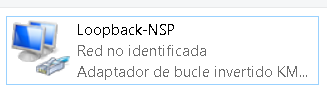
\includegraphics[width=0.55\textwidth]{imagenes/image18.png}
\caption{Adaptador de red Loopback-NSP creado en Windows.}
\end{figure}


Una vez habilitado, se le asignó una dirección IP estática perteneciente a una sebred privada, asegurando que no interfiriera con otras interfaces del equipo.

\subsubsection*{2. Primera topología y modelo de router empleado}

Con el adaptador Loopback configurado, se procedió a crear la primera topología en GNS3. Para ello se utilizó un router Cisco 3660, perteneciente a la plataforma c3600, que ofrecía compatibilidad con comandos IOS y funciones de red básicas. La topología inicial consistía en un único router (R1) conectado directamente al adaptador Loopback mediante el nodo Cloud1), tal como se muestra en la figura \ref{fig:topologia_1}.

\begin{figure}[H]
\centering
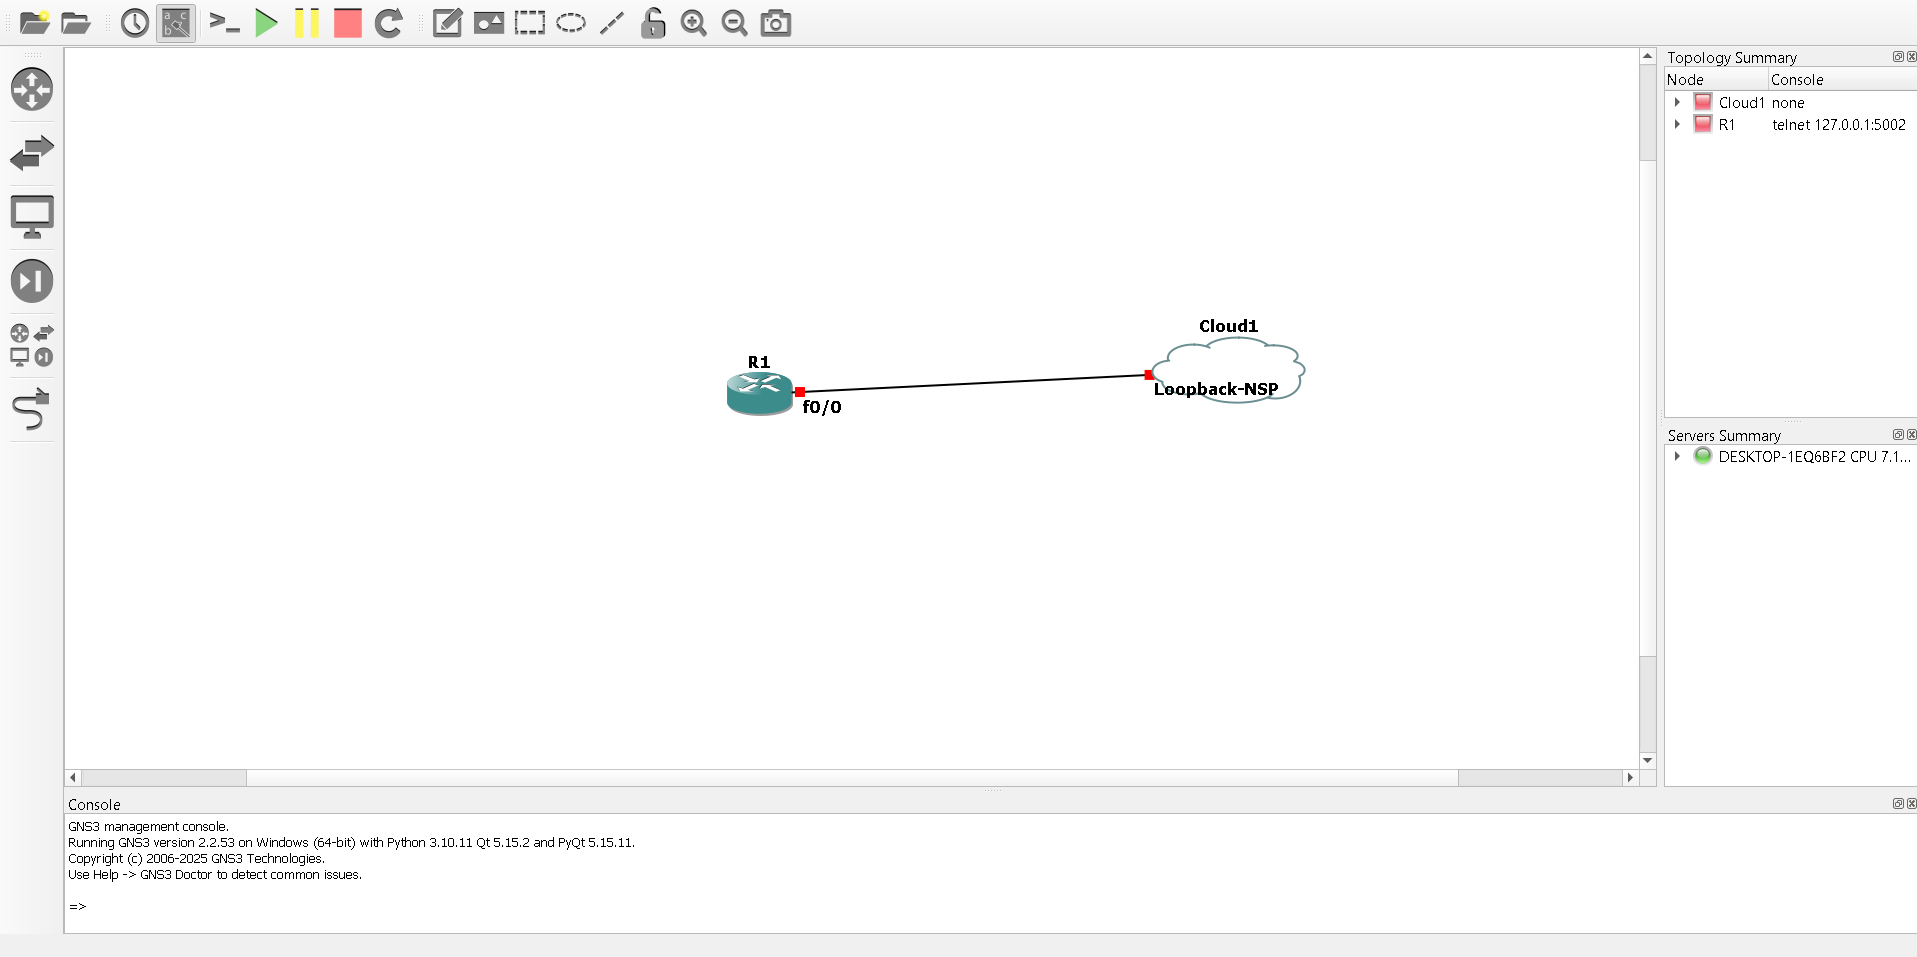
\includegraphics[width=0.9\textwidth]{imagenes/image19.png}
\caption{Topología inicial en GNS3 utilizando el adaptador Loopback-NSP.}
\label{fig:topologia_1}
\end{figure}

El router se configuró a partir de la imagen C3660-JK.BIN, estableciendo el modo consola telnet como interfaz de administración por defecto.

\begin{figure}[H]
\centering
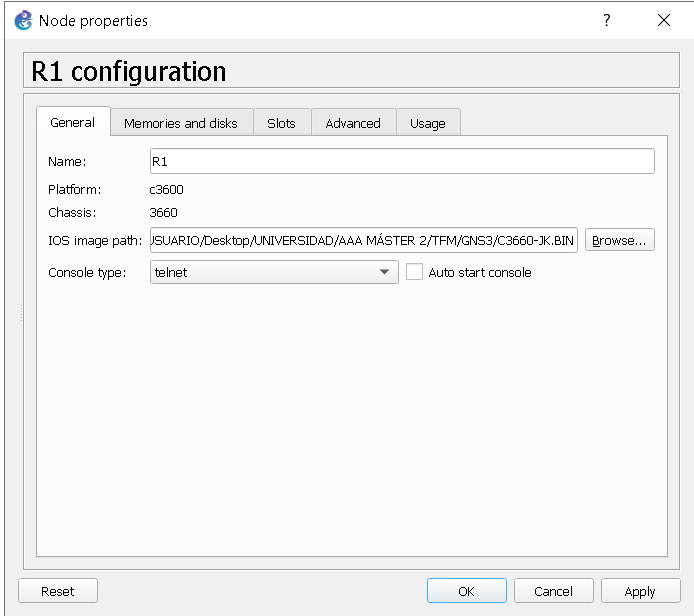
\includegraphics[width=0.7\textwidth]{imagenes/image20.png}
\caption{Configuración del router Cisco 3660 en GNS3.}
\end{figure}

\subsubsection*{3. Asignación de IP y prueba de conectividad}

En esta primera configuración la interfaz FastEthernet0/0 del router se configuró con la direción 192.168.143.1/24, con el objetivo de verificar la comunicación entre ambos dispositivos mediante ICMP.

El comando "show ip interface brief" permitió confirmar que la interfaz del router se encontraba activa:

\begin{figure}[H]
\centering
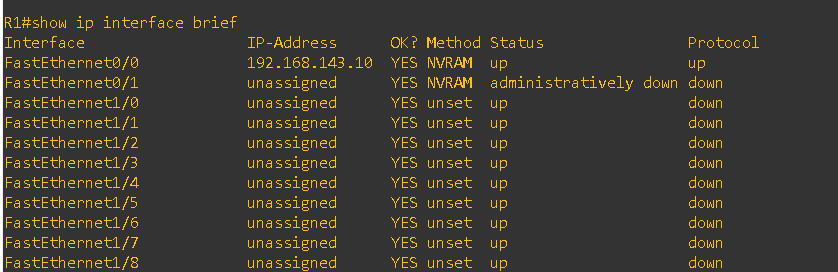
\includegraphics[width=0.85\textwidth]{imagenes/image21.png}
\caption{IP asignada al router Cisco 3660 durante la primera prueba.}
\end{figure}

Sin embargo, la prueba de ping desde el sistema anfitrión a la dirección del router no fue satisfactoria. Como se observa en la figura \ref{fig:ping_fallo}, la conexión devolvía respuestas intermitentes y mensajes de “Host de destino inaccesible”, lo que imedía establecer comunicación bidireccional

\begin{figure}[H]
\centering
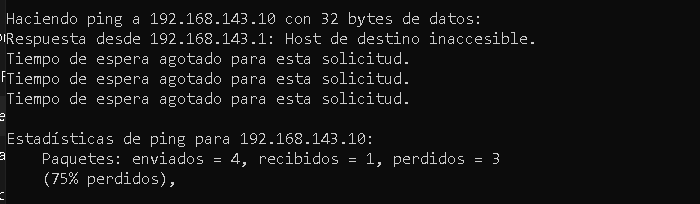
\includegraphics[width=0.8\textwidth]{imagenes/image22.png}
\caption{Resultado de la primera prueba de conectividad entre el adaptador Loopback y el router Cisco.}
\label{fig:ping_fallo}
\end{figure}

\subsubsection*{4. Análisis de las causas del fallo}

Durante varias semanas se realizaron numerosos intentos para resolver este problema, ajustando diferentes parámetros tanto en GNS3 como en el sistema operativo:

\begin{itemize}
    \item Se verificó que el adaptador Loopback estuviera correctamente asociado al nodo Cloud1.
    \item Se probaron distintas configuraciones de direcciones IP y máscaras de subred.
    \item Se modificaron las opciones de red en GNS3 (modo puente, NAT, y host-only) sin obtener resultados satisfactorios.
    \item Se comprobaron posibles conflictos con firewalls o antivirus del sistema.
\end{itemize}

A pesar de estos esfuerzos, la conexión seguía siendo inestable y no se conseguía establecer una comunicación fiable entre el router y el equipo anfitrión. se concluyó que el problema residía en las limitaciones del adaptador Loopback bajo el sistema operativo Windows, que no gestionaba correcatmente la comunicación con los entornos virtualizados de GNS3.

\subsubsection*{5. Transición a un entorno virtual Linux}

Ante la imposibilidad de lograr conectividad de lograr conectividad directa desde Windows, se optó por un enfoque: la creación de una máquina virtual Linux, mediante Oracle VirtualBox, que actuase como intermediaria entre GNS3 y el sistema de desarrollo.

Para ello se instaló una máquina virtual Ubuntu 22.04, la cual serviría posteriormente como servidor del backend FastAPI y pasarela de comunicación con los routers simulados.

\begin{figure}[H]
\centering
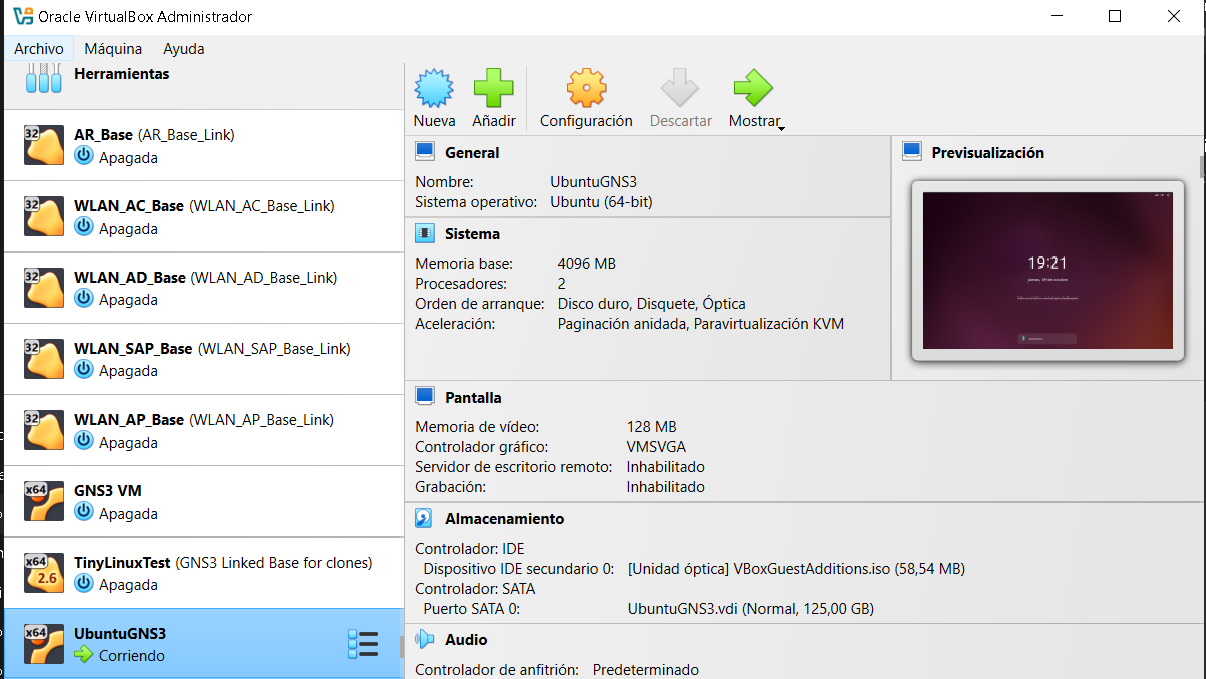
\includegraphics[width=0.9\textwidth]{imagenes/image23.png}
\caption{Máquina virtual Ubuntu creada para gestionar la comunicación con GNS3.}
\end{figure}

Esta máquina se configuró con 4 GB de memoria RAM y dos procesadores, asegurando un rendimiento fluido. El nuevo entorno permitió configurar adaptadores de red específicos y gestionar la comunicación con los routers de forma más controlada.

\subsubsection*{6. Verificación del entorno Linux}

Dentro de la máquina virtual, se asignaron las interfaces de red de forma estática. La interfaz enp0s8 recibió la dirección IP 192.168.56.10/24, mientras que el router se configuró con 192.168.56.2/24. La salida del comando ip a confirmó la correcta configuración de las interfaces.

\begin{figure}[H]
\centering
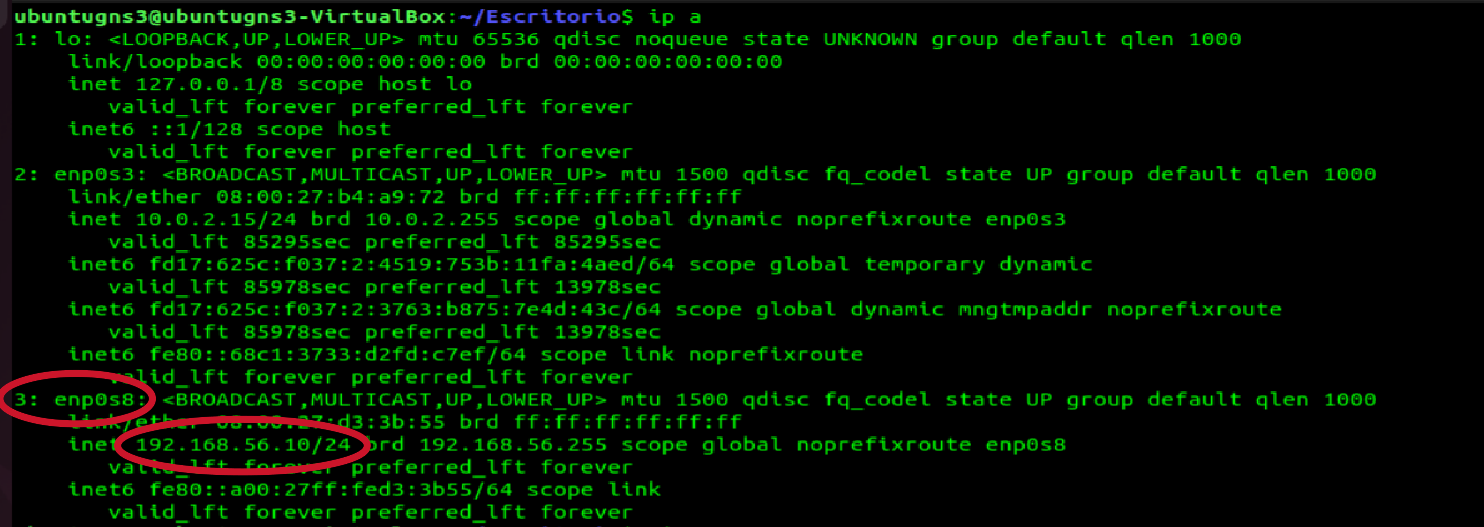
\includegraphics[width=0.95\textwidth]{imagenes/image24.png}
\caption{Direcciones IP configuradas en la máquina virtual Ubuntu.}
\end{figure}

\subsubsection*{7. Validación de la conectividad final}

Finalmente, se realizó una nueva prueba de ping desde Ubuntu hacia el router Cisco, obteniendo una comunicación completamente funcional y estable, como se muestra en la figura \ref{fig:ping_ok}. 

\begin{figure}[H]
\centering
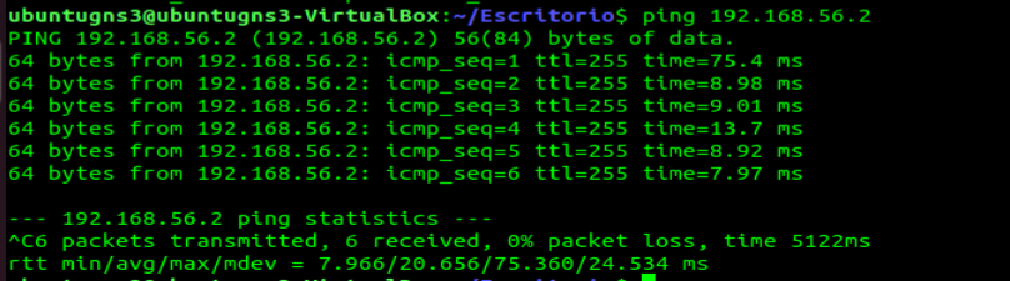
\includegraphics[width=0.85\textwidth]{imagenes/image25.png}
\caption{Prueba de conectividad exitosa entre Ubuntu y el router Cisco.}
\label{fig:ping_ok}
\end{figure}

\subsubsection*{8. Prueba de conectividad SSH con el router}

Con el objetivo de verificar que el protocolo SSH puede emplearse para acceder al router desde la máquina virtual (Ubuntu), se realizó una prueba controlada en la que se configuró el servicio SSH en el dispositivo Cisco y se ejecutó una conexión desde el cliente. A continuación se detallan los pasos, los comandos utilizados en cada terminal y las comprobaciones realizadas.

\begin{itemize}
  \item Router (R1): FastEthernet0/0 = 192.168.56.2/24, estado up/up.
  \item Máquina virtual Ubuntu: enp0s8 = 192.168.56.10/24.
  \item Conectividad L3: ping 192.168.56.2 correcto desde ubuntu.
\end{itemize}

Para habilitar el acceso SSH en IOS es necesario definir \textit{hostname} y \textit{ip domain-name}, generar claves RSA, crear un usuario local y forzar SSH en las líneas VTY. Se emplearon los siguientes comandos:


\begin{lstlisting}[language={},caption={Configuración IOS para habilitar SSH},label={lst:ssh-ios-config}]
R1> enable
R1# configure terminal
! 1) Identidad del dispositivo (requerido para las claves RSA)
R1(config)# hostname R1
R1(config)# ip domain-name red.local

! 2) Generación de claves RSA (tamaño recomendado >= 1024/2048)
R1(config)# crypto key generate rsa modulus 2048
*% Generating 2048 bit RSA keys, keys will be non-exportable...[OK]

! 3) Usuario local con privilegios administrativos
R1(config)# username francisco privilege 15 secret francisco

! 4) Habilitación de SSH v2 y parámetros recomendados
R1(config)# ip ssh version 2
R1(config)# ip ssh time-out 60
R1(config)# ip ssh authentication-retries 3

! 5) Forzar SSH en las líneas virtuales (VTY 0-4)
R1(config)# line vty 0 4
R1(config-line)# login local
R1(config-line)# transport input ssh
R1(config-line)# exec-timeout 10 0
R1(config-line)# exit

! (Opcional) Asegurar la interfaz de gestión activa y sin shutdown
R1(config)# interface FastEthernet0/0
R1(config-if)# ip address 192.168.56.2 255.255.255.0
R1(config-if)# no shutdown
R1(config-if)# exit

! Guardar la configuración
R1(config)# end
R1# write memory
Building configuration...
[OK]
\end{lstlisting}

\noindent
Verificaciones en el router tras la configuración:
\begin{lstlisting}[language={},caption={Comprobaciones rápidas en el router},label={lst:ssh-ios-show}]
R1# show ip ssh
R1# show ssh
R1# show run | section line vty
R1# show users
\end{lstlisting}

En el cliente se comprobó primero la conectividad IP y la apertura del puerto TCP/22. Posteriormente, se estableció la sesión SSH aceptando la huella de la clave del router:

\begin{lstlisting}[language=bash,caption={Pruebas en Ubuntu: ICMP, puerto 22 y acceso SSH},label={lst:ssh-ubuntu}]
# 1) Verificar conectividad IP (ICMP)
ping -c 4 192.168.56.2

# 2) Comprobar que el puerto SSH (22/TCP) está accesible
# Si está disponible netcat (nc):
nc -zv 192.168.56.2 22
# Alternativa con nmap (si está instalado):
# sudo nmap -p 22 192.168.56.2

# 3) Establecer sesión SSH
ssh francisco@192.168.56.2

# Primera conexión: aceptar huella (fingerprint) del host
# Are you sure you want to continue connecting (yes/no/[fingerprint])? yes
# (Introducir la contraseña cuando sea solicitada)
\end{lstlisting}

Como se puede mostrar en la siguiente figura \ref{fig:ssh_ok} la conexión SSH se estableció correctamente desde Ubuntu, con autenticación local en el router y cifrado de la sesión, confirmando que el protocolo SSH queda operativo para su uso por el backend (FastAPI + Paramiko)

\begin{figure}[H]
\centering
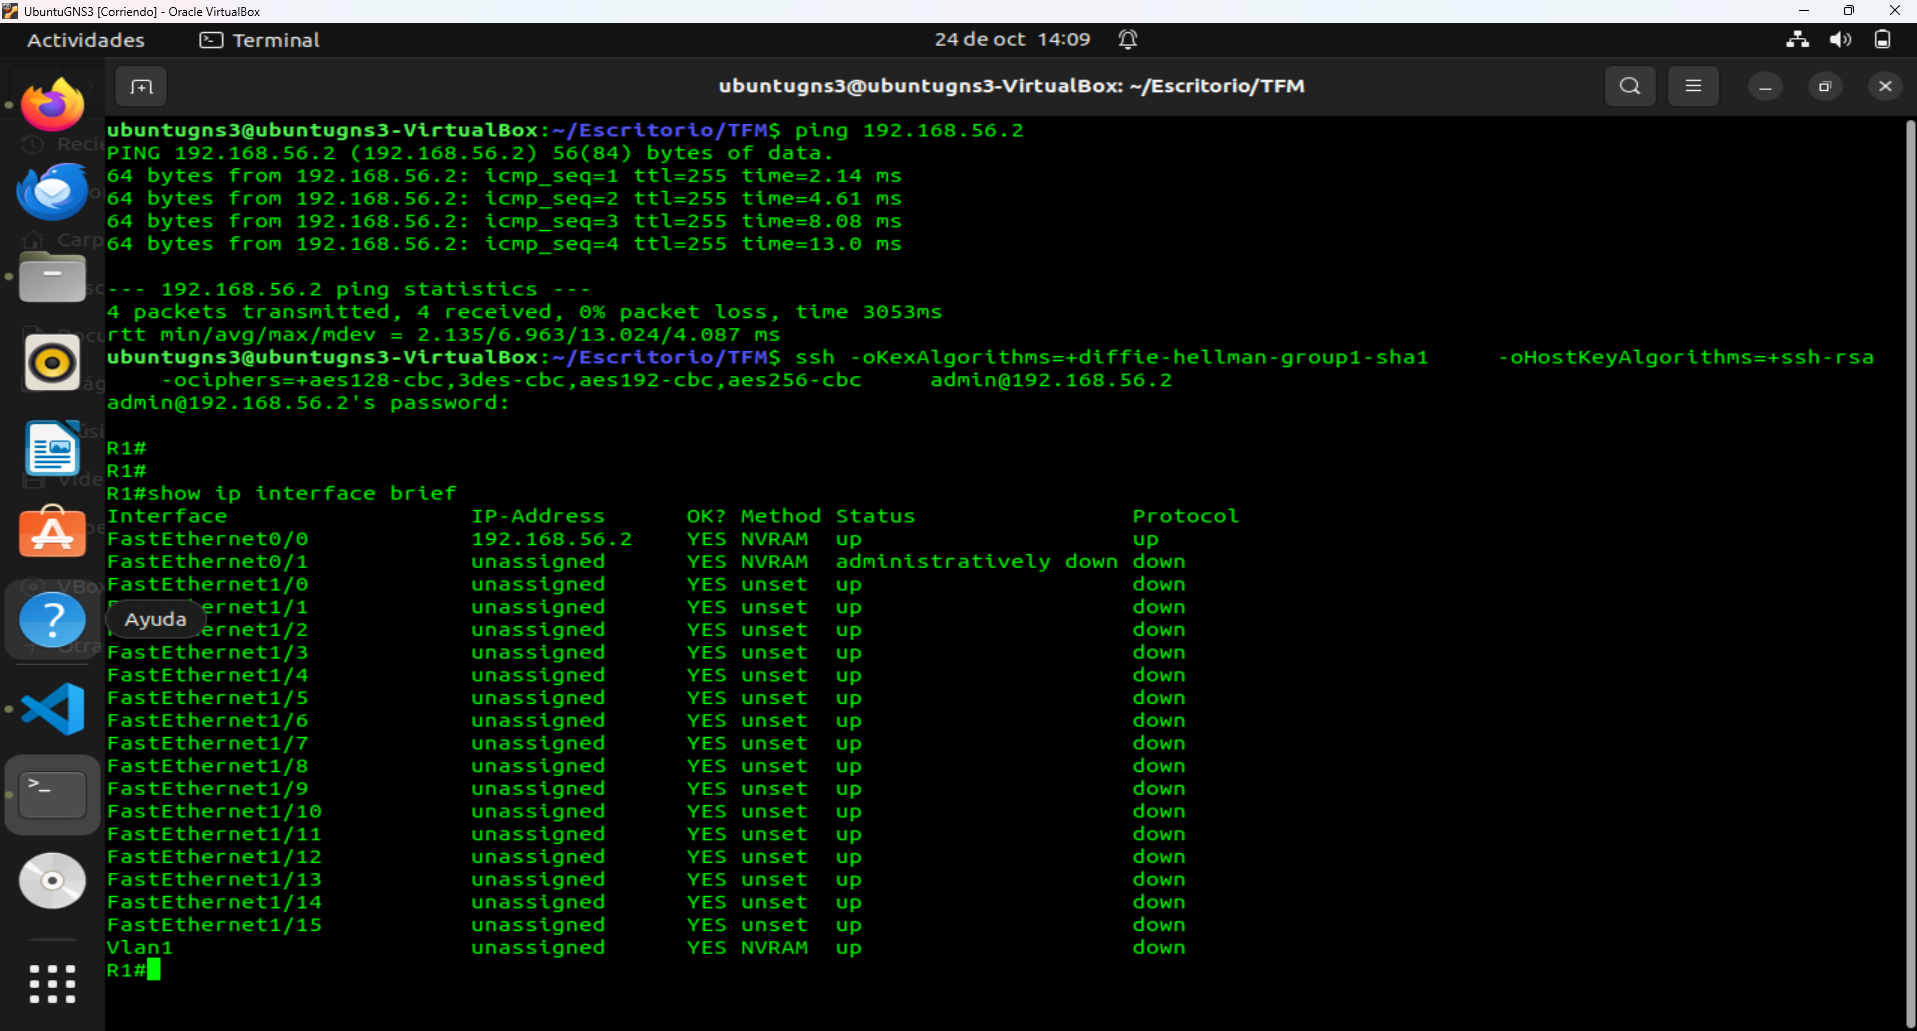
\includegraphics[width=0.9\textwidth]{imagenes/image26.png}
\caption{Prueba de conectividad exitosa entre Ubuntu y el router Cisco.}
\label{fig:ssh_ok}
\end{figure}

\section{Esquema conceptual de la base de datos}

Aunque la versión actual del sistema no incorpora una base de datos relacional para el almacenamiento persistente, resulta necesario definir un esquema conceptual que represente de forma estructurada las entidades fundamentales del sistema. Este modelo conceptual no describe una implementación concreta, si no que proporciona una visión abstracta que facilita la comprensión del dominio del problema, a la vez que establece una base sólida para futura aplicaciones del proyecto en las que se contemple la integración de una base de datos.

A partir del análisis funcional realizado y de las necesidades detectadas en el proceso de monitorización, se han identificado cuatro entidades principales: \textbf{Usuario}, \textbf{Router}, \textbf{Interfaz} y \textbf{ErrorInterfaz}. Estas entidades representan a los actores y elementos clave del sistema, así como las relaciones lógicas entre ellos. La entidad \textbf{Usuario} recoge la información relativa a los usuarios autenticados, mientras que la entidad \textbf{Router} modela los dispositivos de red monitorizados. Cada router dispone de varias interfaces, agrupadas en la entidad \textbf{Interfaz}, y finalmente la entidad \textbf{ErrorInterfaz} recoge los errores o anomalías detectados durante el proceso de monitorización.

En la figura~\ref{fig:esquema_bd} se muestra el esquema conceptual que resume las entidades identificadas y las relaciones existentes entre ellas. Este diagrama proporciona una visión clara del modelo de datos teórico, independientemente de la implementación actual basada en consultas en tiempo real mediante SSH.

\begin{figure}[H]
    \centering
    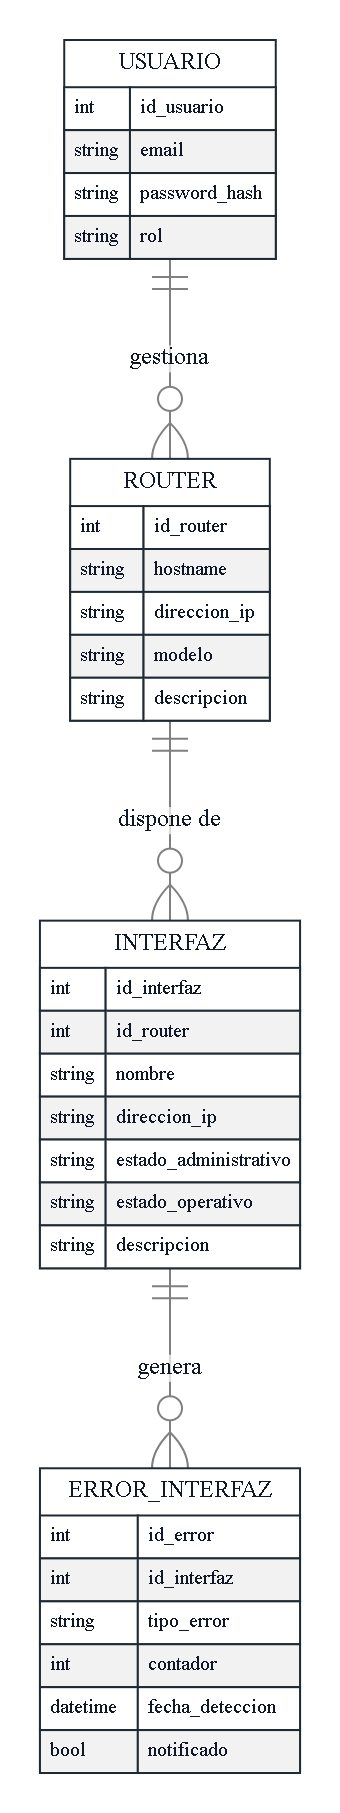
\includegraphics[width=0.25\linewidth]{canva/esquema_bd.png}
    \caption{Esquema conceptual de la base de datos del sistema de monitorización.}
    \label{fig:esquema_bd}
\end{figure}

A continuación se describen con mayor detalle las entidades incluidas en el modelo conceptual:

\begin{itemize}
    \item Usuario. Representa a los usuarios del sistema que acceden mediante un proceso de autenticación. Sus atributos principales incluyen:
    \begin{itemize}
        \item id\_usuario: identificador único del usuario.
        \item email: dirección de correo utilizada para autenticarse.
        \item password\_hash: contraseña cifrada.
        \item rol: tipo de usuario (administrador o usuario estándar).
    \end{itemize}

    \item Router. Esta entidad agrupa la información necesaria para identificar y gestionar los routers monitorizados.
    \begin{itemize}
        \item id\_router: identificador único del router.
        \item hostname: nombre del router.
        \item direccion\_ip: dirección IP de gestión.
        \item modelo: modelo del dispositivo.
        \item descripcion: información adicional asociada al router.
    \end{itemize}

    \item Interfaz. Cada router dispone de múltiples interfaces físicas o lógicas. Esta entidad permite representar la información asociada a cada una de ellas:
    \begin{itemize}
        \item id\_interfaz: identificador único de la interfaz.
        \item id\_router: clave foránea que relaciona la interfaz con su router.
        \item nombre: nombre de la interfaz (p.\,ej.\ FastEthernet0/0).
        \item direccion\_ip: dirección IP configurada en la interfaz.
        \item estado\_administrativo: estado administrativo (up/down).
        \item estado\_operativo: estado real de funcionamiento (up/down).
        \item descripcion: descripción opcional de la interfaz.
    \end{itemize}

    \item ErrorInterfaz. Esta entidad recoge los errores detectados en las interfaces durante la monitorización periódica del sistema.
    \begin{itemize}
        \item id\_error: identificador único del error registrado.
        \item id\_interfaz: referencia a la interfaz donde se ha detectado el error.
        \item tipo\_error: tipo de error (CRC, colisiones, \textit{input errors}, etc.).
        \item contador: valor del contador de errores en el momento de la detección.
        \item fecha\_deteccion: momento exacto de la detección del error.
        \item notificado: indica si el error ha sido incluido en un informe PDF y notificado al usuario.
    \end{itemize}

\end{itemize}


